\documentclass[9pt,a4paper]{article}


\usepackage[russian]{babel}
\usepackage[justification=centering]{caption}
\usepackage[backend=bibtex]{biblatex}
\usepackage{fontspec}
\usepackage{graphicx}
\usepackage{listings}
\usepackage{array}
\usepackage{xcolor}
\usepackage{graphicx}
\usepackage{tikz}
\usepackage{pgfplots}
%\usepackage{geometry}
\graphicspath{{./images/}}

\setmainfont{Spectral Light}%{Times New Roman}

\definecolor{codegreen}{rgb}{0,0.6,0}
\definecolor{codegray}{rgb}{0.5,0.5,0.5}
\definecolor{codepurple}{rgb}{0.58,0,0.82}
\definecolor{backcolour}{rgb}{0.95,0.95,0.92}

\lstdefinestyle{mystyle}{
    backgroundcolor=\color{white},   
    commentstyle=\color{codegreen},
    keywordstyle=\color{magenta},
    numberstyle=\color{codegray},
    stringstyle=\color{codepurple},
    basicstyle=\ttfamily\footnotesize,
    morekeywords={*,procedure, if, rol, cmpj, setmask, then, else, endif, cmpjn, is, not, and, return},            % if you want to add more keywords to the set
    breakatwhitespace=false,         
    breaklines=true,                 
    captionpos=b,                    
    keepspaces=true,                 
    numbers=left,                    
    numbersep=10pt,
    xleftmargin=7mm,
    xrightmargin=0mm,
    showspaces=false,                
    showstringspaces=false,
    showtabs=false,                  
    tabsize=4
}
\lstset{style=mystyle}
\lstset{linewidth=9cm}
\bibliography{asvk} 


\begin{document}
\title{
    Анализ и исследование структур данных для поиска в таблицах классификации 
    в архитектуре сетевого процессора без выделенного ассоциативного устройства
}
\maketitle
    \begin{abstract}
        В данной работе рассматривается проблема классификации пакетов в рамках архитектуры 
        сетевого процессора, без выделенного ассоциативного устройства.
        Под классификацией понимается процесс идентификации пакета по его заголовку.
        Для этапа классификации требуется реализация структур данных для хранения 
        таблиц классификации.
        В рассматриваемом сетевом процессоре присутствуют некоторые ограничения, 
        из-за которых невозвожно использование TCAM памяти.
        На основе ограничений рассматриваемой архитектуры были выбраны 
        структуры данных для дальнейших исследований.
        На основе выбранных структур данных были реализованы адаптированные под рассматриваемую 
        архитектуру сетевого процессора деревья. 
        Экспериментальное исследование, реализованных структур данных, 
        было проведено на имитационной модели сетевого процессора,
        Использование адаптированного АВЛ дерева позволило сократить 
        количество тактов сетевого процессора на обработку одного пакета 
        и уменьшить использование памяти вычислительных блоков конвейера.
    \end{abstract}
    
    \section{Введение}
        В настоящее время активно развивается технология программно-конфигурируемых 
        сетей~\cite{smel2012open}, в которых требуются высокопроизводительные 
        коммутаторы~\cite{bifulco2018survey}. Возникает задача разработки 
        программируемого сетевого процессора, являющегося основным функциональным 
        элементом коммутаторов. Сетевой процессор представляет из себя интегральную 
        микросхему, специализированную для обработки сетевых пакетов, которая выполняет следующие функции:
        получение пакета с физического порта, выделение заголовка,
        классификация пакета по его заголовку, принятие решения о дальнейшем 
        пути следования пакета, отправка пакета на физический порт~\cite{chao2007high:1}.
        В настоящее время активно ведётся разработка программируемых сетевых процессоров. 
        Под программируемым сетевым процессором понимается сетевой процессор, 
        который позволяет менять программу обработки пакетов и набор различаемых 
        полей заголовков, что позволяет быстро подстраиваться под новые протоколы, 
        и использовать коммутатор в ПКС сетях~\cite{bezzubtsev2019ob-odnom183708319}.
        
        Исходя из функций сетевого процессора, целесообразно рассматривать архитектуру, основанную на
        наборе конвейеров, которая позволяет с фиксированной задержкой обрабатывать каждый пакет. 
        Конвейер в сетевом процессоре состоит из вычислительных блоков. В данной работе рассматривался этап классификации пакетов. 
        Под классификацией понимается процесс идентификации сетевого пакета по его признакам, определяемыми текущим протоколом.
        Таблица классификации $-$ набор правил, содержащих в себе признаки, по которым идентифицируется группа пакетов,
        и действия, которые сетевой процессор выполняет над данной группой пакетов. 
        Таким образом, для выполнения классификации сетевой процессор должен включать в себя ассоциативное устройство. Для реализации этого устройства естественным будет использование 
        ассоциативной памяти. Однако единственный контроллер ассоциативной памяти будет являться узким местом, так как к нему должны иметь доступ все стадии всех конвейера.
        Соответственно, возникает потребность усложнения архитектуры, например, путём добавления в неё нескольких контроллеров ассоциативной памяти.
        Чтобы избежать сложной организации памяти, в архитектуре можно отказаться от использования ассоциативной памяти. 
        В таком случае одно из решений $-$ совместить память команд и данных, и разместить память на кристалле сетевого процессора.
        Таким образом, возникает задача разработки структур данных для поиска в таблицах классификации в сетевом процессоре без выделенного ассоциативного устройства.
    \section{Архитектура сетевого процессора}
        \label{section:problem}
        В рассматриваемом сетевом процессоре используется конвейерная архитектура, каждый конвейер состоит из 10 вычислительных блоков. 
         
        Каждый вычислительный блок имеет доступ к участку памяти, в котором располагаются микрокод и данные.
        Существует ограничение на количество тактов, которое один пакет может обрабатываться на вычислительном блоке, оно соответствует 25 тактам.
        Данное ограничение обусловлено требованием к производительности сетевого процессора, а именно требованием фиксированного времени обработки одного пакета на сетевом процессоре.
        Также один вычислительный блок имеет доступ к 2 мегабайтам памяти.
        Из-за особенностей микроархитектуры, отсутствует отдельная область памяти, в которой хранятся данные. Поэтому микрокод содержит в себе все данные,
        необходимые для классификации пакетов.

        \begin{figure}[h]
            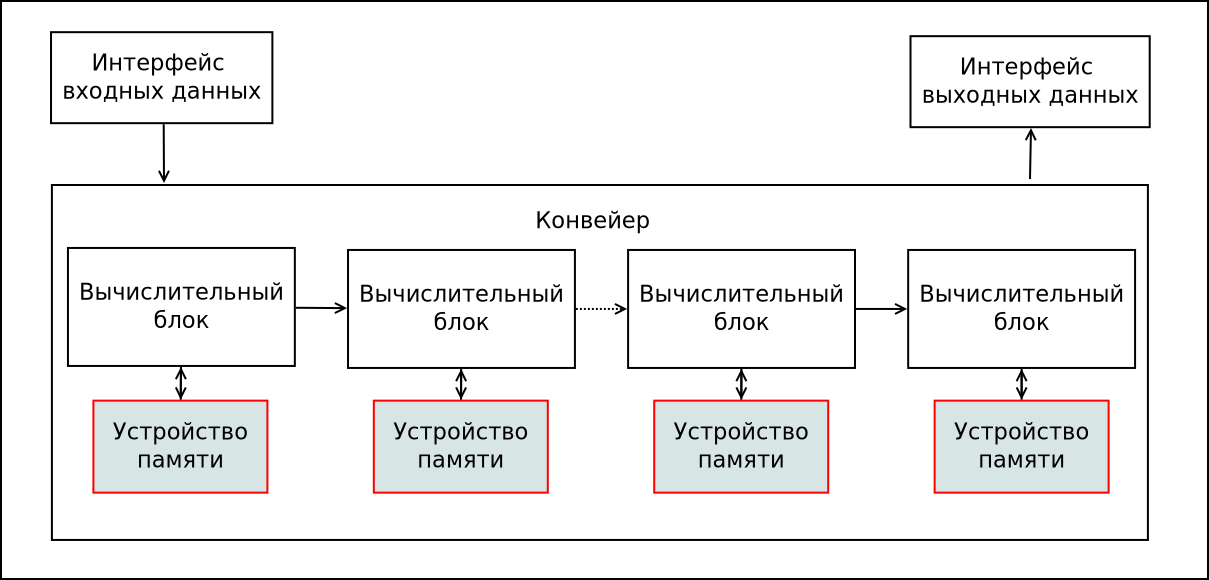
\includegraphics[width=0.5\textwidth]{npu_all.png}
            %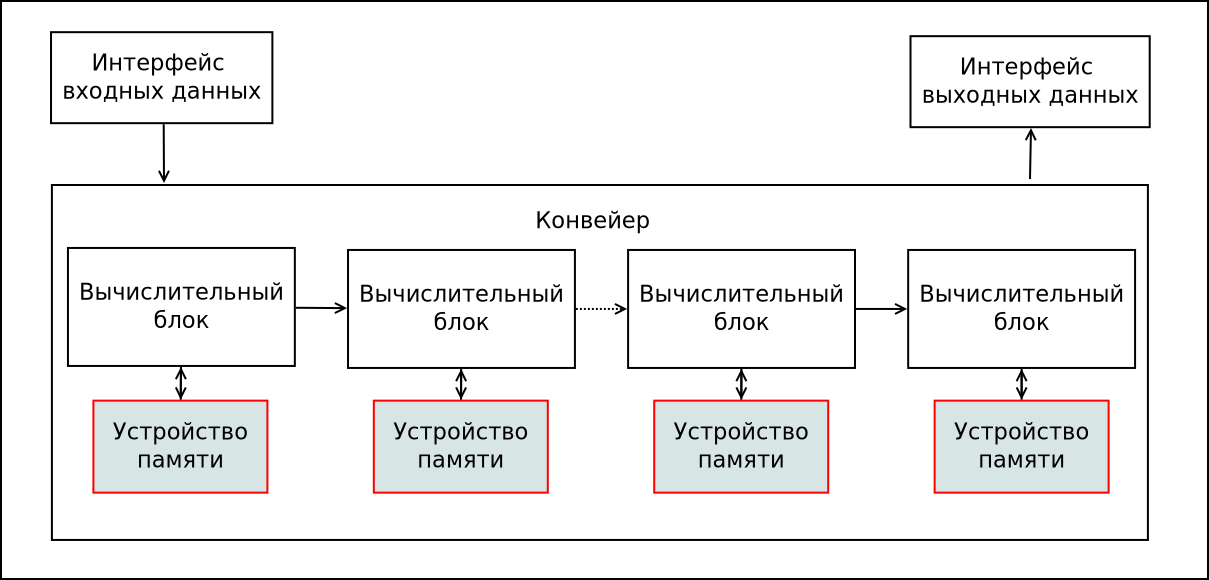
\includegraphics[]{npu_all.png}
            \caption{Архитектура рассматриваемого сетевого процессора}
        \end{figure}
        
        \subsection{Язык ассемблера сетевого процессора}
            Для описания программ обработки сетевых пакетов в рассматриваемой архитектуре сетевого процессора используется язык ассемблера. 
            В рассматриваемом языке присутствуют следующие классы инструкций:
            \begin{itemize}
                \item Инструкции для работы с регистром.
                \item Инструкции арифметических операций.
                \item Инструкции битовых операций.
                \item Инструкции для условного и безусловного перехода на метку.
                \item Инструкция записи в регистр выходного порта.
            \end{itemize}
    \section{Проделанная работа}
        В литературе представлены решения поставленой задачи. 
        В силу особенностей архитектуры сетевого процессора, а именно отсутствия 
        адресуемой памяти, 
        которая требуется для не древовидных структур данных будут рассматриваться 
        только древовидные структуры данных. 
        
        В рассматриваемых решениях будут рассматриваться следующие аспекты:
        {\bf асимптотическая сложность поиска} $-$ позволяет оценить использование 
        ресурсов сетевого процессора для поиска в структуре данных,
        {\bf универсальность структуры данных} $-$ используемая структура данных
        должна поддерживать поиск произвольных битовых строк, не превосходящих по длине 128 бит,
        {\bf необходимость использования адресуемой памяти} $-$ некоторым рассматриваемым 
        структурам данных требуется адресуемая память для их реализации, 
        соответствующей их асимптотической сложности,
        {\bf количество вершин}, которое необходимо посетить для поиска
        в случае хранения битовых строк длиной до 48 бит,
        {\bf необходимость изменения микроархитектуры} вычислительных блоков конвейера 
        сетевого процессора,
        {\bf оценка объёма памяти}, занимаемой структурой данных $-$ рассматривается объём памяти, занимаемый структурой данных, для 64000 вхождений префиксов IPv4.
        В рассматриваемой литературе используется несколько основных подходов к разработке структур данных, 
        для хранения таблиц классификации. А именно: использование принципа хеш таблиц, использование принципа деревьев 
        и использование принципа балансирующихся деревьев.

    \subsection{Метод подсчёта объёма памяти занимаемый рассматриваемой структурой данных}
        Для реализуемой структуры данных вычисляется количество вершин для хранения 64000 битовых строк $-$ $N$, затем вычисляется среднее количество инструкций на 
        одну вершину $-$ $S$. Тогда искомый объём памяти занимаемый структурой данных будет рассчитываться по формуле $M = instruction\_size * N * S$,
        где $instruction\_size = 128$, в силу рассматриваемой архитектуры сетевого процессора.
    \subsection{Использование хеш таблиц}
        Данный подход использует адресуемую память, поэтому в данной работе он не рассматривался. 
        Так как в рассматриваемой архитектуре сетевого процессора отсутствует возможность адресуемой памяти.
        Одним из примеров такого подходя является бинарный поиск по длинам префиксов.
        Рассматриваемая структура данных основана на построении специальных таблиц для префиксов определённой длины~\cite{mun2006binary}. 
        Пусть максимальная длина префикса {\ttfamily $W$}, тогда строятся таблицы {\ttfamily $h_{1},\ldots,h_{w}$}. 
        В каждой из них хранятся префиксы длины соответствующие номеру этой таблицы. 
        Предполагается, что в каждой такой таблице реализована своя хеш-функция, 
        которая быстро позволяет найти вхождение префикса в данную таблицу.
        Таким образом мы можем выполнить бинарный поиск по длине префиксов. 
        В рамках рассматриваемой архитектуры сетевого процессора, 
        реализация таких таблиц возможна только с использованием древовидных структур данных~\cite{mun2006binary}. 

    \subsection{использование деревьев}
        \label{section:bctrev}
            Наиболее распространенная~\cite{behdadfar2009scalar} структура данных для поиска по 
            наибольшему совпадению это бинарное однобитное дерево. 
            Строится дерево по заданным префиксам так, что каждому биту префикса соответствует своя вершина в дереве. 
            Поиск осуществляется спуском в глубину по битам элемента, для которого выполняется поиск. 
            Поиск заканчивается тогда, когда достигнута пустая вершина, результатом поиска считается последний встретившийся префикс~\cite{chao2007high:1}.
            Оптимизацией бинарного однобитного дерева~\cite{ruiz2001survey} является бинарное сжатое дерево. 
            Для построения данного дерева необходимо построить бинарное однобитное дерево, 
            затем провести процедуру сжатия, а именно все вершины, у которых только один лист, 
            сокращаются, и в следующую вершину заносятся данные о количестве пропущенных вершин. 
            Таким образом, построенное дерево не имеет вершин с одним листом. 
            Благодаря описанной оптимизации, данное дерево занимает меньше памяти, 
            чем бинарное однобитное дерево. Это обусловлено отсутствием проходных вершин. 
            Однако, уменьшается количество затраченных инструкций на поиск лишь 
            для префиксов, перед которыми были однолистные вершины. Для худшего случая, когда для префикса есть все его более короткие версии, количество вершин, 
            которые нужно посетить для поиска, аналогично бинарному однобитному дереву ~\cite{ruiz2001survey}. 

            Мультибитное сжатое дерево $-$ оптимизация бинарного сжатого дерева~\cite{berger2003ip}.
            Используется другая структура деревьев, когда в каждой вершине может быть максимум не два листа, 
            а {\ttfamily $2^h$}, где {\ttfamily $h$} $-$ это максимальная глубина поддерева данной вершины.
            При использовании рассматриваемой структуры данных в рамках архитектуры процессора общего назначение, 
            количество операций для поиска ограничивается глубиной дерева,
            которая равна {\ttfamily $\frac{W}{K}$}, где {\ttfamily $W$} $-$ длина максимального префикса, 
            а {\ttfamily $K$} $-$ количество уровней в нашем дереве.
            В рамках архитектуры сетевого процессора будет рассматриваться реализация данного дерева, 
            в которой используется линейный поиск в каждой вершине по дочерним вершинам~\cite{berger2003ip}.
                    
        \subsection{Использование балансирующихся деревьев}
            \label{section:avlrev}
            В данной категории в литературе рассматривалось много различних балансирующихся деревьев, таких как: В-деревья,
            красно-черные деревья, АВЛ дерево. Во всех балансирующихся деревьях используется алгоритм представления префиксов
            как скалярных величин.
            В данной работе в качестве примера подробно рассматривалось АВЛ дерево.
            Представление префиксов как скалярных префиксов позволяет использовать больший набор структур данных~\cite{behdadfar2009scalar}. 
            В качестве примера рассмотрим АВЛ дерево, основной особенностью которого является правило его построения: у каждой вершины разность 
            глубины левого и правого поддерева не превосходит 1, что даёт асимптотическую сложность поиска {\ttfamily $O(1+\log_2{N})$}, 
            где {\ttfamily $N$} $-$ количество префиксов в нашей структуре данных. Из этого следует, что время поиска не зависит от длины искомых данных,
            а значит с помощью данной структуры данных эффективно выполнять поиск префиксов IPv6~\cite{behdadfar2011coded}.
            \\
    \subsection{Сравнение структур данных}
        У каждой рассмотренной структуры данных есть свои достоинства и недостатки, рассмотрим их:
        \begin{enumerate}
            \item \textbf{Бинарное однобитное дерево} $-$ данная структура проста в реализации, но занимает много памяти и поиск требует прохождения 48 вершин.
            \item \textbf{Бинарное сжатое дерево} $-$ занимает меньше памяти, чем двоичное однобитное дерево, но поиск требует прохождения 48 вершин. 
                Соответственно использование данного дерева предпочтительнее, чем двоичного однобитного дерева.
            \item \textbf{Мультибитное сжатое дерево} $-$ занимает много памяти, но поиск требует прохождения сильно меньшего количества вершин. 
                Из-за проблем с реализацией в рамках рассматриваемой архитектуры, эта структура данных не может быть реализована.
            \item \textbf{Бинарный поиск по длинам префиксов} $-$ занимает много памяти, и может быть использован только для поиска наиболее длинного префикса.
                Также из-за проблем с реализацией на рассматриваемой архитектуре, данная структура не подходит для решения проблемы.
            \item \textbf{АВЛ дерево} $-$ занимает меньше всего памяти, и при этом, поиск требует прохождения малого количества вершин,
                которое зависит от количества вхождений в структуру данных, а не от конкретного префикса.
        \end{enumerate}

        Таким образом на основе обзора для дальнейшей реализации целесообразно выбрать две структуры данных: 
        АВЛ дерево с алгоритмом представления префиксов как скалярных величин и бинарное сжатое дерево. 
        Также в качестве эталона выбрано бинарное однобитное дерево.

\section{Предложенные структуры данных}
        \label{section:trees}
        В описании алгоритмов использовалась структура данных \emph{Node}, которая содержит в себе следующие поля:
        \begin{itemize}
            \item \emph{Node.left} $-$ ссылка на левого сына вершины.
            \item \emph{Node.right} $-$ ссылка на правого сына вершины.
            \item \emph{Node.rule} $-$ действие, соответствующее префиксу данной вершины.
            \item \emph{Node.prefix} $-$ префикс в текущей вершине.
            \item \emph{Node.bit} $-$ значащий бит в текущей вершине.
        \end{itemize}
        И структура \emph{prefix}, которая содержит в себе следующие поля:
        \begin{itemize}
            \item \emph{prefix.bit\_string} $-$ битовая строка, задающая префикс.
            \item \emph{prefix.length} $-$ длина префикса. При поиске точного совпадения длина префикса равна длине битовой строки.
        \end{itemize}

        \subsection{Бинарное однобитное дерево}
        \label{section:binone}
            Рассмотрим алгоритм построения бинарного однобитного дерева, являющийся базовым для бинарнго сжатого дерева.
            Для добавления вершин в структуру данных определим процедуру \emph{Add} (Листинг~\ref{lst1}).\\
            {\bf Входные данные:} текущая вершина \emph{Node}, добавляемый префикс \emph{prefix}, правило для текущего префикса \emph{rule}, и текущий бит \emph{bit}.\\
            {\bf Выходные данные:} обновлённая текущая вершина, а именно объект структуры \emph{Node}.
\\
\begin{lstlisting}[caption=Процедура добавления вершины в бинарное однобитное дерево., label=lst1]
procedure Add(Node, prefix, rule, bit)
    if Node is empty then
        Node = new Node()
        Node.bit = bit
    endif
    if prefix.length == bit then
        Node.prefix = prefix
        Node.rule = rule
        Node.bit = bit
        return Node
    endif
    if prefix.bit_string[bit] == 1 then
        Node.left = Add(Node.left, prefix, rule, bit + 1)
    else
        Node.right = Add(Node.right, prefix, rule, bit + 1)
    endif
    return Node
\end{lstlisting}
\vspace{1em}
            Таким образом, для построения бинарного однобитного дерева необходимо последовательно добавить все правила из таблицы классификации,
            используя процедуру \emph{Add}.

        \subsection{Бинарное сжатое дерево}
            Рассмотрим алгоритм построения бинарного сжатого дерева. Для упрощения программной реализации сначала строилось бинарное однобитное дерево,
            процедура построения которого описана в пункте~\ref{section:binone}. Для получения из построенного бинарного однобитного дерева бинарного сжатого дерева,
            необходимо удалить все вершины, которые имеют только одного сына, и не имеют префикса.
            \subsubsection{Процедура удаления незначимых вершин}
                Рассмотрим процедуру удаления \emph{Remove} незначимых вершин из бинарного однобитного дерева, для получения бинарного сжатого дерева.\\
                {\bf Входные данные:} текущая вершина \emph{Node}.\\
                {\bf Выходные данные:} обновлённая текущая вершина \emph{Node}.
                Алгоритм удаления не важных вершин может быть представлен в виде псевдокода процедуры \emph{Remove} (Листинг~\ref{lst2})
\\
\begin{center} 
\begin{lstlisting}[caption=Процедура удаления незначимых вершин., label=lst2]
procedure Remove(Node):
    if Node.prefix is empty then
        if Node.left is empty and Node.right is not empty then
            return Node.right
        endif
        if Node.left is not empty and Node.right is empty then
            return Node.left
        endif
    else
        return Node
    endif
\end{lstlisting}
\end{center}
\vspace{1em}
            Данный алгоритм позволяет построить бинарное сжатое дерево, на базе бинарного однобитного дерева, путём удаления незначимых вершин из бинарного однобитного дерева.\\
            Для данного дерева необходимо было разработать процедуру описывающую вершину рассматриваемой структуры данных. Данная процедура должна позволять выполнять
            поиск по построенной структуре данных.
            Рассмотрим процедуру описывающую вершину двоичного сжатого дерева в рамках рассматриваемой архитектуры сетевого процессора:
\\
\begin{lstlisting}[caption=Процедура описывающая вершину бинарном сжатом дереве.]
setmask (1 << port)
cmpj lable, prefix.bit_string, prefix.length
\end{lstlisting}
\vspace{1em}
            В данной процедуре: 
            \emph{setmask 1 <\,< port} $-$ является опциональной инструкцией и присутствует только тогда, когда в текущей вершине содержится префикс.
            \emph{cmpj label, prefix.bit\_string, prefix.length} $-$ сравнение в текущей вершине, то происходит переход на метку \emph{label}, иначе просто продолжается выполнение программы.
            Метка \emph{label} $-$ может быть перед левым сыном, если он есть иначе метка \emph{finish}, 
            которая завершает программу и тем самым прекращает поиск по структуре данных.
        \subsection{АВЛ дерево}
            \subsubsection{Алгоритм представления префиксов как скалярных величин}
                Данный алгоритм необходим для сохранения и поиска префиксов в АВЛ дерева, так как изначально в вершинах дерева могут хранится только скалярные величины.
                Алгоритм позволяет сравнивать префиксы между собой~\cite{behdadfar2011coded}, а именно:
                \begin{itemize}
                    \item Если длины двух префиксов совпадают, то они сравниваются как две скалярные величины.
                    \item Если длина префикса $q$ меньше длины префикса $p$, то как скалярные величины сравниваются первые $len(q) - 1$ бит у обоих префиксов.
                \end{itemize}
                Данный алгоритм может быть описан процедурой \emph{PrefixCompare} (Листинг~\ref{lst3}).\\
                {\bf Входные данные:} префикс \emph{prefix1} и префикс \emph{prefix2}.\\
                {\bf Выходные данные:} \emph{True}, если первый префикс больше второго, иначе \emph{False}.
\\
\begin{lstlisting}[caption=Процедура сравнения префиксов как скалярных величин., label=lst3]
procedure PrefixCompare(prefix1, prefix2):
    if prefix1.length == prefix2.length then
        return Int(prefix1.bit_string) > Int(prefix2.bit_string)
    else
        minimal_length = Min(prefix1.length, prefix2.length) - 1
        return Int(prefix1.bit_string[0:minimal_length]) > Int(prefix2.bit_string[0:minimal_length])
    endif
\end{lstlisting}
            \subsubsection{Алгоритм построения дерева} 
                Рассмотрим алгоритм построения АВЛ дерева, а именно добавления в него новых вершин. Данный алгоритм может быть описан процедурой \emph{Add} (Листинг~\ref{lst4}).
                Для построения АВЛ дерева используется структура \emph{Node}, которая идентична структуре описанной в пункте~\ref{section:binone}.\\
                {\bf Входные данные:}
                \begin{itemize}
                    \item \emph{Node} $-$ объект структуры вершины АВЛ дерева.
                    \item \emph{prefix} $-$ текущий префикс.
                    \item \emph{rule} $-$ правило для текущего префикса.
                \end{itemize}
                {\bf Выходные данные:} обновлённая текущая вершина \emph{Node}.\\
                Также в процедуре \emph{Add} используется процедура \emph{BalanceNode}, которая выполняет операцию балансировки АВЛ дерева.\\
\begin{lstlisting}[caption=Процедура добавления вершины в АВЛ дерево., label=lst4]
procedure Add(Node, prefix, rule):
    if Node.prefix is empty then
        return new Node(prefix, rule, depth=1)
    endif
    
    if prefixCompare(prefix, Node.prefix) then
        Node.right = Add(Node.right, prefix, rule)
    else:
        Node.left = Add(Node.left, prefix, rule)
    endif
    
    return BalanceNode(Node)
\end{lstlisting}
\vspace{1em}
    Данная процедура позволяет построить АВЛ дерево, последовательно добавляя правила из таблицы.
    \section{Экспериментальное исследование}
    \subsection{Имитационная модель сетевого процессора}
        Имитационная модель сетевого процессора $-$ программное средство написанное на языке программирования python, которая позволяет имитировать работу сетевого процессора, 
        а именно получать пакеты на любой из 24-х портов, обрабатывать пакет, получая информацию о любой стадии обработки, и отправлять пакет на выходные порты.
        Имитационная модель сетевого процессора позволяет оценить количество тактов затраченных на обработку пакета, а также объём памяти, затраченный на структуру данных.
        
        Передача пакетов на порты сетевого процессора осуществляется с помощью файлов $pcap$, в которых можно описать поступление пакетов на каждый порт в определённые моменты времени.
        В данной работе, не ограничивая общности, будет рассматриваться только один порт имитационной модели сетевого процессора. Так как для каждого входного
        порта используется соответствующий конвейер. В конвейере имитационной модели сетевого процессора реализован один вычислительный блок, этого достаточно для проведения 
        экспериментального исследование, так как конвейер сетевого процессора имеет статическое расписание.

        Исходная программа для обработки пакетов принимается в виде кода, написанного на языке ассемблера, который используется в рассматриваемой архитектуре сетевого процессора.
        Имитационная модель преобразует программу, раскрывая директивы $\#include$ и $\#define$, и начинает имитацию работы сетевого процессора по этой программе.
        
        
    \subsection{Описание программной реализации}
        Для проведения дальнейшего экспериментального исследования необходимо разработать программную реализацию на языке python. Программная реализация должна включать в себя
        следующие модули:
        
        \begin{itemize}
            \item Модуль загрузки таблиц классификации из файла.
            \item Модуль построения АВЛ-дерева.
            \item Модуль построения Бинарного сжатого дерева.
            \item Модуль построения Бинарного однобитного дерева.
            \item Модуль преобразования построенного дерева в язык ассемблера.
        \end{itemize}
        Схема взаимодействия модулей представлена на рисунке~\ref{fig:mesh5}.
       
        \begin{figure}[ht]
            \centering
            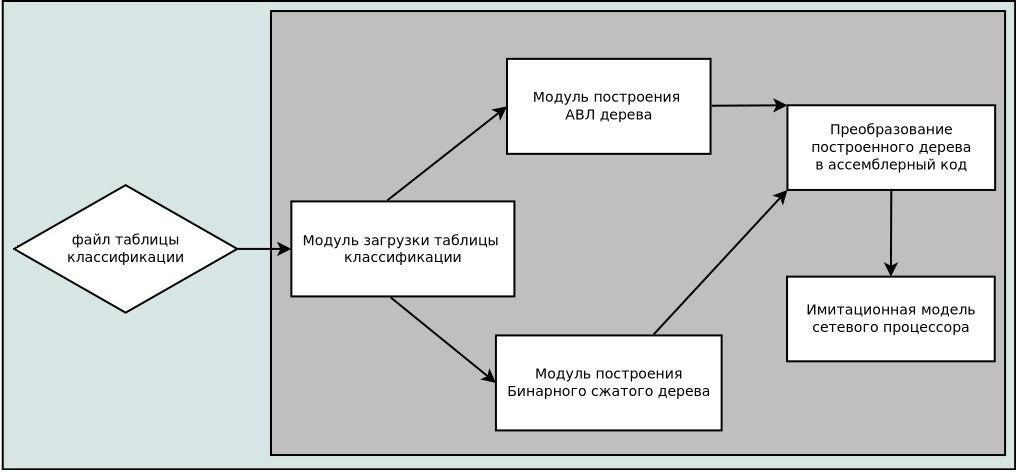
\includegraphics[width=0.5\textwidth]{program_scheme.jpg}
            \caption{Схема программной реализации}\label{fig:mesh5}
        \end{figure}        

        \subsubsection{Модуль загрузки таблиц классификации}
            \label{section:tablemod}
            В данном модуле реализуется считывание файлов таблиц классификации и преобразование их в словарь где ключом является битовая строка,
            по которой будет происходить поиск, а значением номер порта коммутатора. Данные словари отправляются в модули построения структур данных.
            Модуль позволяет использовать существующие таблицы классификации для проведения экспериментального исследования.
            Пример входных таблиц классификации представлен в листинге~\ref{lst6}\\
\begin{lstlisting}[caption=Пример таблиц классификации, label=lst6]
{IPv4}
192.168.31.0 24 1
192.168.43.0 24 2
\end{lstlisting}
        \subsubsection{Модули построения структур данных}
            В данных модулях реализуется построение описанных деревьев, а именно, бинарного сжатого дерева, бинарного однобитного дерева и АВЛ дерева.
            На вход модули принимают считанные из файла и преобразованные таблицы классификации.
            Затем каждое правило последовательно добавляется в структуру данных, алгоритм добавления описан в главе~\ref{section:trees}, для каждой из 
            рассматриваемых структур данных.
            После построения структура данных передаётся в модуль преобразования дерева в язык ассемблера использующийся в сетевом процессоре в виде корневой вершины.
            
        \subsubsection{Модуль построения преобразования построенного дерева на язык ассемблера}
            Для каждого дерева модуль преобразования строит определённый ассемблерный код, подробно описанный в главе~\ref{section:trees}.
            Преобразование происходит рекурсивно проходя древовидную структуру данных, вершины последовательно записываются в массив, и затем
            для каждой вершины генерируется собственный ассемблерный код.
            Сгенерированный ассемблерный код записывается в указанный файл. Затем файл используется при экспериментальном исследовании на имитационной модели сетевого процессора.
            Пример преобразования бинарного сжатого дерева из пункта~\ref{section:bctrev} представлен в листинге~\ref{lst7}.\\
\begin{lstlisting}[caption=Пример бинарного сжатого дерева на языке ассемблера., label=lst7]
cmpj l_1, 1, 1
setmask (1 << 3)
cmpjn finish, 1, 2
setmask (1 << 1)
j finish

l_1:
cmpj l_2, 11, 2
cmpjn finish, 101, 3
setmask (1 << 5)
cmpjn finish, 1011, 4
setmask (1 << 6)
j finish

l_2:
setmask (1 << 4)
cmpjn finish, 1100, 4
setmask (1 << 2)
j finish

finish:
\end{lstlisting}

    \subsection{Методика экспериментального исследования}
            Для проведения экспериментального исследования были найдены таблицы коммутации префиксов различной длины. Экспериментальное исследование будет проводится
            для таблиц классификации различного размера, а именно: 1000, 8000, 16000, 32000, 64000 битовых строк. Будут использоваться битовые строки различной длины, а именно:
            32, 48 бита. Для каждой структуры данных будут проведены исследования с трафиком покрывающим загруженную таблицу в имитационную модель сетевого процессора.
            Также будет проводится исследование с поиском наиболее длинного префикса и точного совпадения.
            
            Для проведения экспериментального исследования необходимо выполнить следующие действия:
            \begin{enumerate}
                \item Подготовить входные данные для программной реализации, а именно привести таблицы классификации к виду описанному в пункте~\ref{section:tablemod}.
                \item Для каждой из рассматриваемых таблиц классификации построить разработанные структуры данных и преобразовать их в ассемблерный код.
                \item Провести имитацию для каждой структуры данных на имитационной модели сетевого процессора.
                \item Зафиксировать полученные данные при имитации, а именно объём затраченной памяти конвейера сетевого процессора, и среднее количество инструкций
                    на классификацию пакета.
            \end{enumerate}

            Для бинарного сжатого дерева ожидается получить значительное уменьшение объёма памяти и уменьшение среднего количества тактов на один пакет 
            по сравнению с бинарным однобитным деревом.
            Для АВЛ дерева ожидается уменьшение среднего количества тактов затраченных на поиск одного пакета по сравнению с бинарным сжатым деревом и 
            не сильное уменьшение затраченного объёма памяти на хранение структуры данных.
    \section{Результаты экспериментального исследования}
        В данной главе представлены результаты экспериментального исследования разработанных структур данных для таблиц классификации размера от 1000 до 64000, 
        и признаками различной длины.
        \subsection{Бинарное однобитное дерево}
            Рассмотрим график зависимости среднего количества инструкций, потраченных на поиск по структуре данных, для пакета от количества правил в таблице классификации (Рис.~\ref{graph:btinst}).
            \begin{figure}[!htbp]
                \centering
            \begin{tikzpicture}
            \begin{axis}[
                width=0.7\textwidth,
                height=0.7\textwidth,
                ylabel={Количество инструкций},
                xlabel={Количество правил},
                y label style={at={(-0.05, 0.5)}},
                ymin=25, ymax=60,
                xmin=1000, xmax=64000,
                xmode=log,
                log basis x={2},
                xtick={0, 128, 256, 512, 1024, 2048, 4096, 8192, 16384, 32768},
                ytick={30, 35, 40, 45, 50, 55},
                legend pos=south east,
                ymajorgrids=true,
                grid style=dashed,
                cycle list name=color list] 
                \addplot+[mark=square] coordinates{(1000, 46)(8000, 47)(16000, 48)(32000, 48)(64000, 48)};
                \addplot+[mark=square] coordinates{(1000, 30)(8000, 37)(16000, 40)(32000, 43)(64000, 47)};
                \legend{32 бит, 48 бит}
            \end{axis}
            \end{tikzpicture}
                \captionsetup{justification=centering}
                \caption{Зависимость количества инструкций от количества правил.}
                \label{graph:btinst}
            \end{figure}
            Как видно из представленного графика, среднее количество затраченных инструкций практически не изменяется в зависимости от размера таблицы классификации. 
            В среднем количество составляет 48 инструкций на пакет для битовых строк длины 32 бита, и в среднем 41 инструкцию для битовых строк длины 48 бит.
            Теперь рассмотрим график зависимости затраченного объёма памяти от количества правил в таблице классификации (Рис.~\ref{graph:btmem}).
            \begin{figure}[!htbp]
                \centering
            \begin{tikzpicture}
            \begin{axis}[
                width=0.7\textwidth,
                height=0.7\textwidth,
                ylabel={Память [КБайт]},
                xlabel={Количество правил},
                y label style={at={(-0.05, 0.5)}},
                ymin=0, ymax=7000,
                xmin=1000, xmax=64000,
                xmode=log,
                log basis x={2},
                xtick={0, 128, 256, 512, 1024, 2048, 4096, 8192, 16384, 32768},
                ytick={0, 1000, 2000, 3000, 4000, 5000, 6000},
                legend pos=south east,
                ymajorgrids=true,
                grid style=dashed,
                cycle list name=color list] 
                \addplot+[mark=square] coordinates{(1000, 328.64)(8000, 1966.62)(16000, 3258.27)(32000, 6045.09)};
                \addplot+[mark=square] coordinates{(1000, 1255.16)(8000, 9287.18)};
                \legend{32 бит, 48 бит}
     
            \end{axis}
            \end{tikzpicture}
                \captionsetup{justification=centering}
                \caption{Зависимость объёма памяти от количества правил.}
                \label{graph:btmem}
            \end{figure}
            Из представленного графика видно, что бинарное однобитное дерево занимает в несколько раз  больше памяти, чем в представленных в главе~\ref{section:problem} ограничениях. 
            Что не позволяет использовать использовать данную структуру данных в рассматриваемой архитектуре сетевого процессора.
        \subsection{Бинарное сжатое дерево}
            Рассмотрим график зависимости среднего количества инструкций, потраченных на поиск по структуре данных, для пакета от количества правил в таблице классификации (Рис.~\ref{graph:compinst}).
            \begin{figure}[h!]
                \centering
            \begin{tikzpicture}
            \begin{axis}[
                width=0.4\textwidth,
                height=0.4\textwidth,
                ylabel={Number of instructions},
                xlabel={Number of rules},
                y label style={at={(-0.05, 0.5)}},
                ymin=15, ymax=50,
                xmin=1000, xmax=64000,
                xmode=log,
                log basis x={2},
                xtick={0, 128, 256, 512, 1024, 2048, 4096, 8192, 16384, 32768},
                ytick={20, 25, 30, 35, 40, 45},
                legend pos=south east,
                ymajorgrids=true,
                grid style=dashed,
                cycle list name=color list] 
                \addplot+[mark=square] coordinates{(1000, 32)(8000, 38)(16000, 40)(32000, 42)(64000, 44)};
                \addplot+[mark=square] coordinates{(1000, 24)(8000, 30)(16000, 32)(32000, 34)(64000, 36)};
                \legend{32 bits, 48 bits}
     
            \end{axis}
            \end{tikzpicture}
                \captionsetup{justification=centering}
                \caption{Dependence number of instructions from number of rules.}
                \label{graph:compinst}
            \end{figure}
            Как видно из представленного графика, среднее количество затраченных инструкций практически не изменяется в зависимости от размера таблицы классификации. 
            В среднем количество составляет 39 инструкций на пакет для битовых строк длины 32 бита, и в среднем 31 инструкцию для битовых строк длины 48 бит.
            Теперь рассмотрим график зависимости затраченного объёма памяти от количества правил в таблице классификации (Рис.~\ref{graph:compmem}).
            \begin{figure}[!htbp]
                \centering
            \begin{tikzpicture}
            \begin{axis}[
                width=0.4\textwidth,
                height=0.4\textwidth,
                ylabel={Memmory [Kbyte]},
                xlabel={Number of rules},
                y label style={at={(-0.05, 0.5)}},
                ymin=0, ymax=7000,
                xmin=1000, xmax=64000,
                xmode=log,
                log basis x={2},
                xtick={0, 128, 256, 512, 1024, 2048, 4096, 8192, 16384, 32768},
                ytick={0, 1000, 2000, 3000, 4000, 5000, 6000},
                legend pos=south east,
                ymajorgrids=true,
                grid style=dashed,
                cycle list name=color list] 
                \addplot+[mark=square] coordinates{(1000, 123.58)(8000, 904.71)(16000, 1709.80)(32000, 3174.94)(64000, 6135.29)};
                \addplot+[mark=square] coordinates{(1000, 133.13)(8000, 1060.78)(16000, 2124.25)(32000, 4247.97)(64000, 8497.06)};
                \legend{32 bits, 48 bits}
     
            \end{axis}
            \end{tikzpicture}
                \captionsetup{justification=centering}
                \caption{Dependence of memory from number of rules.}
                \label{graph:compmem}
            \end{figure}
            Из представленного графика видно, что бинарное сжатое дерево занимает больше памяти, чем в представленных в главе~\ref{section:problem} ограничениях, только при 32000
            правил в таблицах классификации.
        
        \subsection{АВЛ дерево}
            Рассмотрим график зависимости среднего количества инструкций, потраченных на поиск по структуре данных, для пакета от количества правил в таблице классификации (Рис.~\ref{graph:avlinst}).
            \begin{figure}[ht]
                \centering
            \begin{tikzpicture}
            \begin{axis}[
                width=0.4\textwidth,
                height=0.4\textwidth,
                ylabel={Number of instructions},
                xlabel={Number of rules},
                y label style={at={(-0.05, 0.5)}},
                ymin=10, ymax=45,
                xmin=1000, xmax=64000,
                xmode=log,
                log basis x={2},
                xtick={0, 128, 256, 512, 1024, 2048, 4096, 8192, 16384, 32768},
                ytick={15, 20, 25, 30, 35, 40, 45},
                legend pos=south east,
                ymajorgrids=true,
                grid style=dashed,
                cycle list name=color list] 
                \addplot+[mark=square] coordinates{(1000, 24)(8000, 29)(16000, 31)(32000, 33)(64000, 35)};
                \addplot+[mark=square] coordinates{(1000, 21)(8000, 23)(16000, 23)(32000, 24)(64000, 24)};
                \legend{32 bits, 48 bits}
     
            \end{axis}
            \end{tikzpicture}
                \captionsetup{justification=centering}
                \caption{Dependence number of instructions from number of rules.}
                \label{graph:avlinst}
            \end{figure}
            \\
            Как видно из представленного графика, среднее количество затраченных инструкций практически не изменяется в зависимости от размера таблицы классификации. 
            В среднем количество составляет 30 инструкций на пакет для битовых строк длины 32 бита, и в среднем 23 инструкцию для битовых строк длины 48 бит.
            Теперь рассмотрим график зависимости затраченного объёма памяти от количества правил в таблице классификации (Рис.~\ref{graph:avlmem}).
            \\
            \begin{figure}[ht]
                \centering
            \begin{tikzpicture}
            \begin{axis}[
                width=0.4\textwidth,
                height=0.4\textwidth,
                ylabel={Memmory [Kbyte]},
                xlabel={Number of rules},
                y label style={at={(-0.05, 0.5)}},
                ymin=0, ymax=7000,
                xmin=1000, xmax=64000,
                xmode=log,
                log basis x={2},
                xtick={0, 128, 256, 512, 1024, 2048, 4096, 8192, 16384, 32768},
                ytick={0, 1000, 2000, 3000, 4000, 5000, 6000},
                legend pos=north west,
                ymajorgrids=true,
                grid style=dashed,
                cycle list name=color list] 
                \addplot+[mark=square] coordinates{(1000, 36.75)(8000, 273.48)(16000, 528.73)(32000, 1013.71)(64000, 2042.61)};
                \addplot+[mark=square] coordinates{(1000, 69.32)(8000, 553.59)(16000, 1107.23)(32000, 2213.89)(64000, 4429.01)};
                \legend{32 bits, 48 bits}
     
            \end{axis}
            \end{tikzpicture}
                \captionsetup{justification=centering}
                \caption{Dependence of memory from number of rules.}
                \label{graph:avlmem}
            \end{figure}
            \\
            Из представленного графика видно, что АВЛ дерево укладывается в представленные в главе~\ref{section:problem} ограничения, за исключением случая, 
            когда в таблице классификации 64000 правила, с признаками длиной 48 бит. 
        \subsection{Сравнение структур данных}
            В данном пункте представлено сравнение реализованных структур данных. Рассмотрим сравнительные графики всех реализованных структур данных.
            На первом графике (Рис.~\ref{graph:allinst}) представлено сравнение реализованных структур данных по среднему количеству инструкций на один пакет. Видно, что АВЛ дерево показывает лучший результат
            из всех реализованных структур данных.
            \\
            \begin{figure}[ht]
                \centering
            \begin{tikzpicture}
            \begin{axis}[
	            x tick label style={
		        /pgf/number format/1000 sep=},
                height=0.6\textwidth,
                width=0.6\textwidth,
	            ylabel=Количество инструкций,
                xlabel=Бит,
	            enlargelimits=0.05,
	            legend style={at={(0.5,-0.25)},
	            anchor=north,legend columns=3},
	            ybar interval=0.7,
            ]
                \addplot coordinates {(32, 48)(48, 41)(64, 23)};
                \addplot coordinates {(32, 39)(48, 31)(64, 23)};
                \addplot coordinates {(32, 30)(48, 23)(64, 23)};
                \legend{BT, BCT, AVL}
            \end{axis}
            \end{tikzpicture}
                \captionsetup{justification=centering}
                \caption{Compare number of instructions from bits in prefix}
                \label{graph:allinst}
            \end{figure}
            \\
            На следующем графике представлено сравнение реализованных структур данных по максимальному объёму памяти занимаемому структурой данных (Рис.~\ref{graph:allmem}). Видно, что только АВЛ дерево удовлетворяет
            ограничением представленным в пункте~\ref{section:problem}, и занимает значительно меньше памяти, чем остальные структуры данных.
            \\
            \begin{figure}[ht]
                \centering
            \begin{tikzpicture}
            \begin{axis}[
	            x tick label style={
		        /pgf/number format/1000 sep=},
                height=0.6\textwidth,
                width=0.6\textwidth,
	            ylabel=Максимальный объём памяти,
                xlabel=Бит,
	            enlargelimits=0.05,
	            legend style={at={(0.5,-0.25)},
	            anchor=north,legend columns=3},
	            ybar interval=0.7,
            ]
                \addplot coordinates {(32, 74231)(48, 13082)(64, 23)};
                \addplot coordinates {(32, 6532)(48, 8497)(64, 23)};
                \addplot coordinates {(32, 2042.61)(48, 4429.01)(64, 23)};
                \legend{BT, BCT, AVL}
            \end{axis}
            \end{tikzpicture}
                \captionsetup{justification=centering}
                \caption{Comparison of the maximum amount of memory occupied by data structures.}
                \label{graph:allmem}
            \end{figure}
            \\
    \section{Заключение}
        В данной работе была рассмотрена проблема классификации пакетов в рассматриваемой архитектуре сетевого процессора. 
        Были разработаны структуры данных для классификации пакетов в рассматриваемой архитектуре.
        В рамках данной работы были достигнуты следующие результаты:
        \begin{itemize}
            \item Был проведён обзор существующих решений, целью которого было выбрать структуры данных для дальнейшей адаптации и реализации в рамках рассматриваемой архитектуры сетевого процессора. 
                На основе обзора были выбраны АВЛ дерево и бинарное сжатое дерево. 
            \item Выбранные структуры данных были адаптированны под рассматриваемую архитектуру сетевого процессора.
            \item Адаптированные структуры данных были реализованы с использованием языка программирования $python$.
            \item Также были разработаны дополнительные программные средства, для проведения экспериментального исследования.
            \item Было проведено экспериментальное исследование, в результате которого были получены характеристики исследуемых структур данных.
                Для АВЛ дерева дерева $-$ максимальный объём памяти, занимаемый структурой данных,  не превосходит 2 МБ, а среднее количество
                инструкций на классификацию одного пакета равно 30 и 23 для битовых строк длины 32 и 48 бита соответственно.
                Для Бинарного сжатого дерева $-$  максимальный объём памяти, занимаемый структурой данных,  не превосходит  8.5 МБ, а среднее количество
                инструкций на классификацию одного пакета равно 39 и 31 для битовых строк длины 32 и 48 бита соответственно.
            \item Из полученных данных при проведении экспериментального исследования был сделан вывод, что только АВЛ дерево удовлетворяет ограничениям,
                поставленным в данной работе.
        \end{itemize}

        В качестве направления дальнейших исследований, можно указать исследование возможности дальнейшей оптимизации реализованных структур данных, 
        для уменьшения объёма занимаемой памяти структурами данных, а также рассмотрение изменений архитектуры сетевого процессора
        и структур, которые требуют изменений в рассматриваемой архитектуре.

 

\end{document}
